\section{还未解决的问题}
    \subsection{短测例}
    \par
    考虑如下这么一个例子
    \begin{center}
        $\bar{x_{1}} \cup \bar{x_{2}} \cup \bar{x_{3}}$
    \end{center}
    \par
    这是理论上应该给出的结果
    \begin{figure}[H]
        \centering
        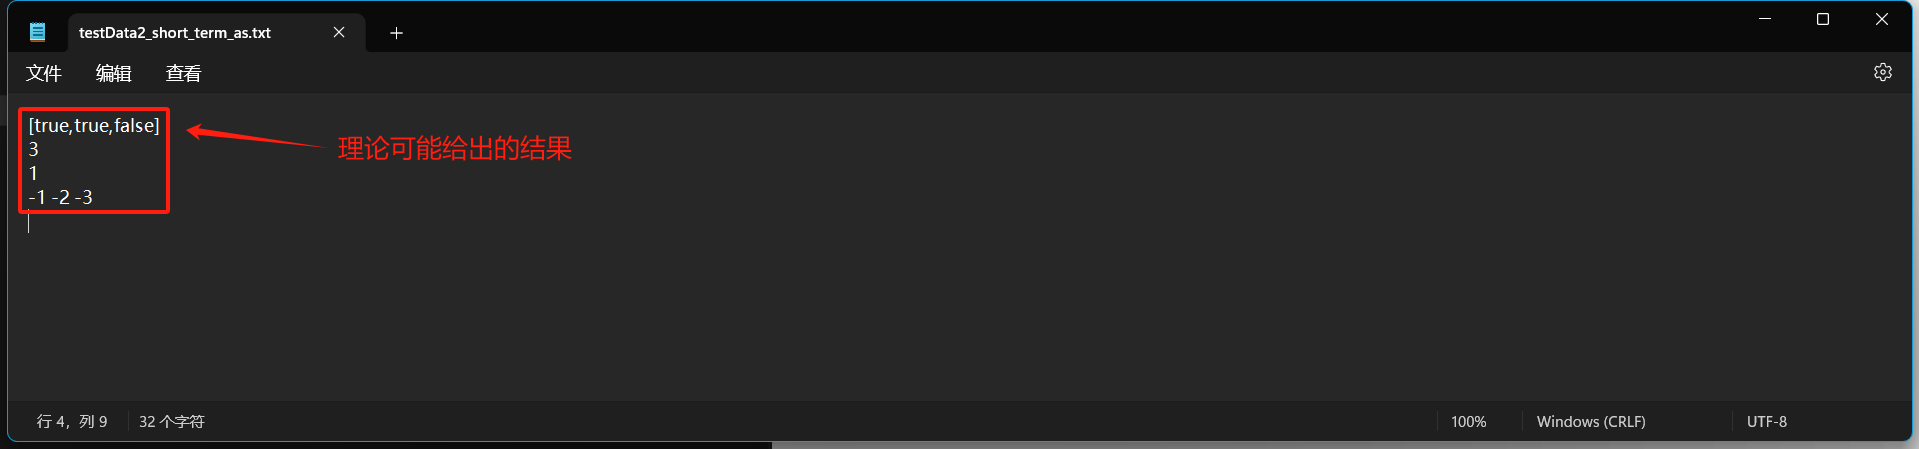
\includegraphics[width=10cm]{Figure/Figure_4.jpg}
        \caption{理论上求解短测例应该得出的结果}
    \end{figure}
    \par
    这是利用回溯法求解短测例给出的结果
    \begin{figure}[H]
        \centering
        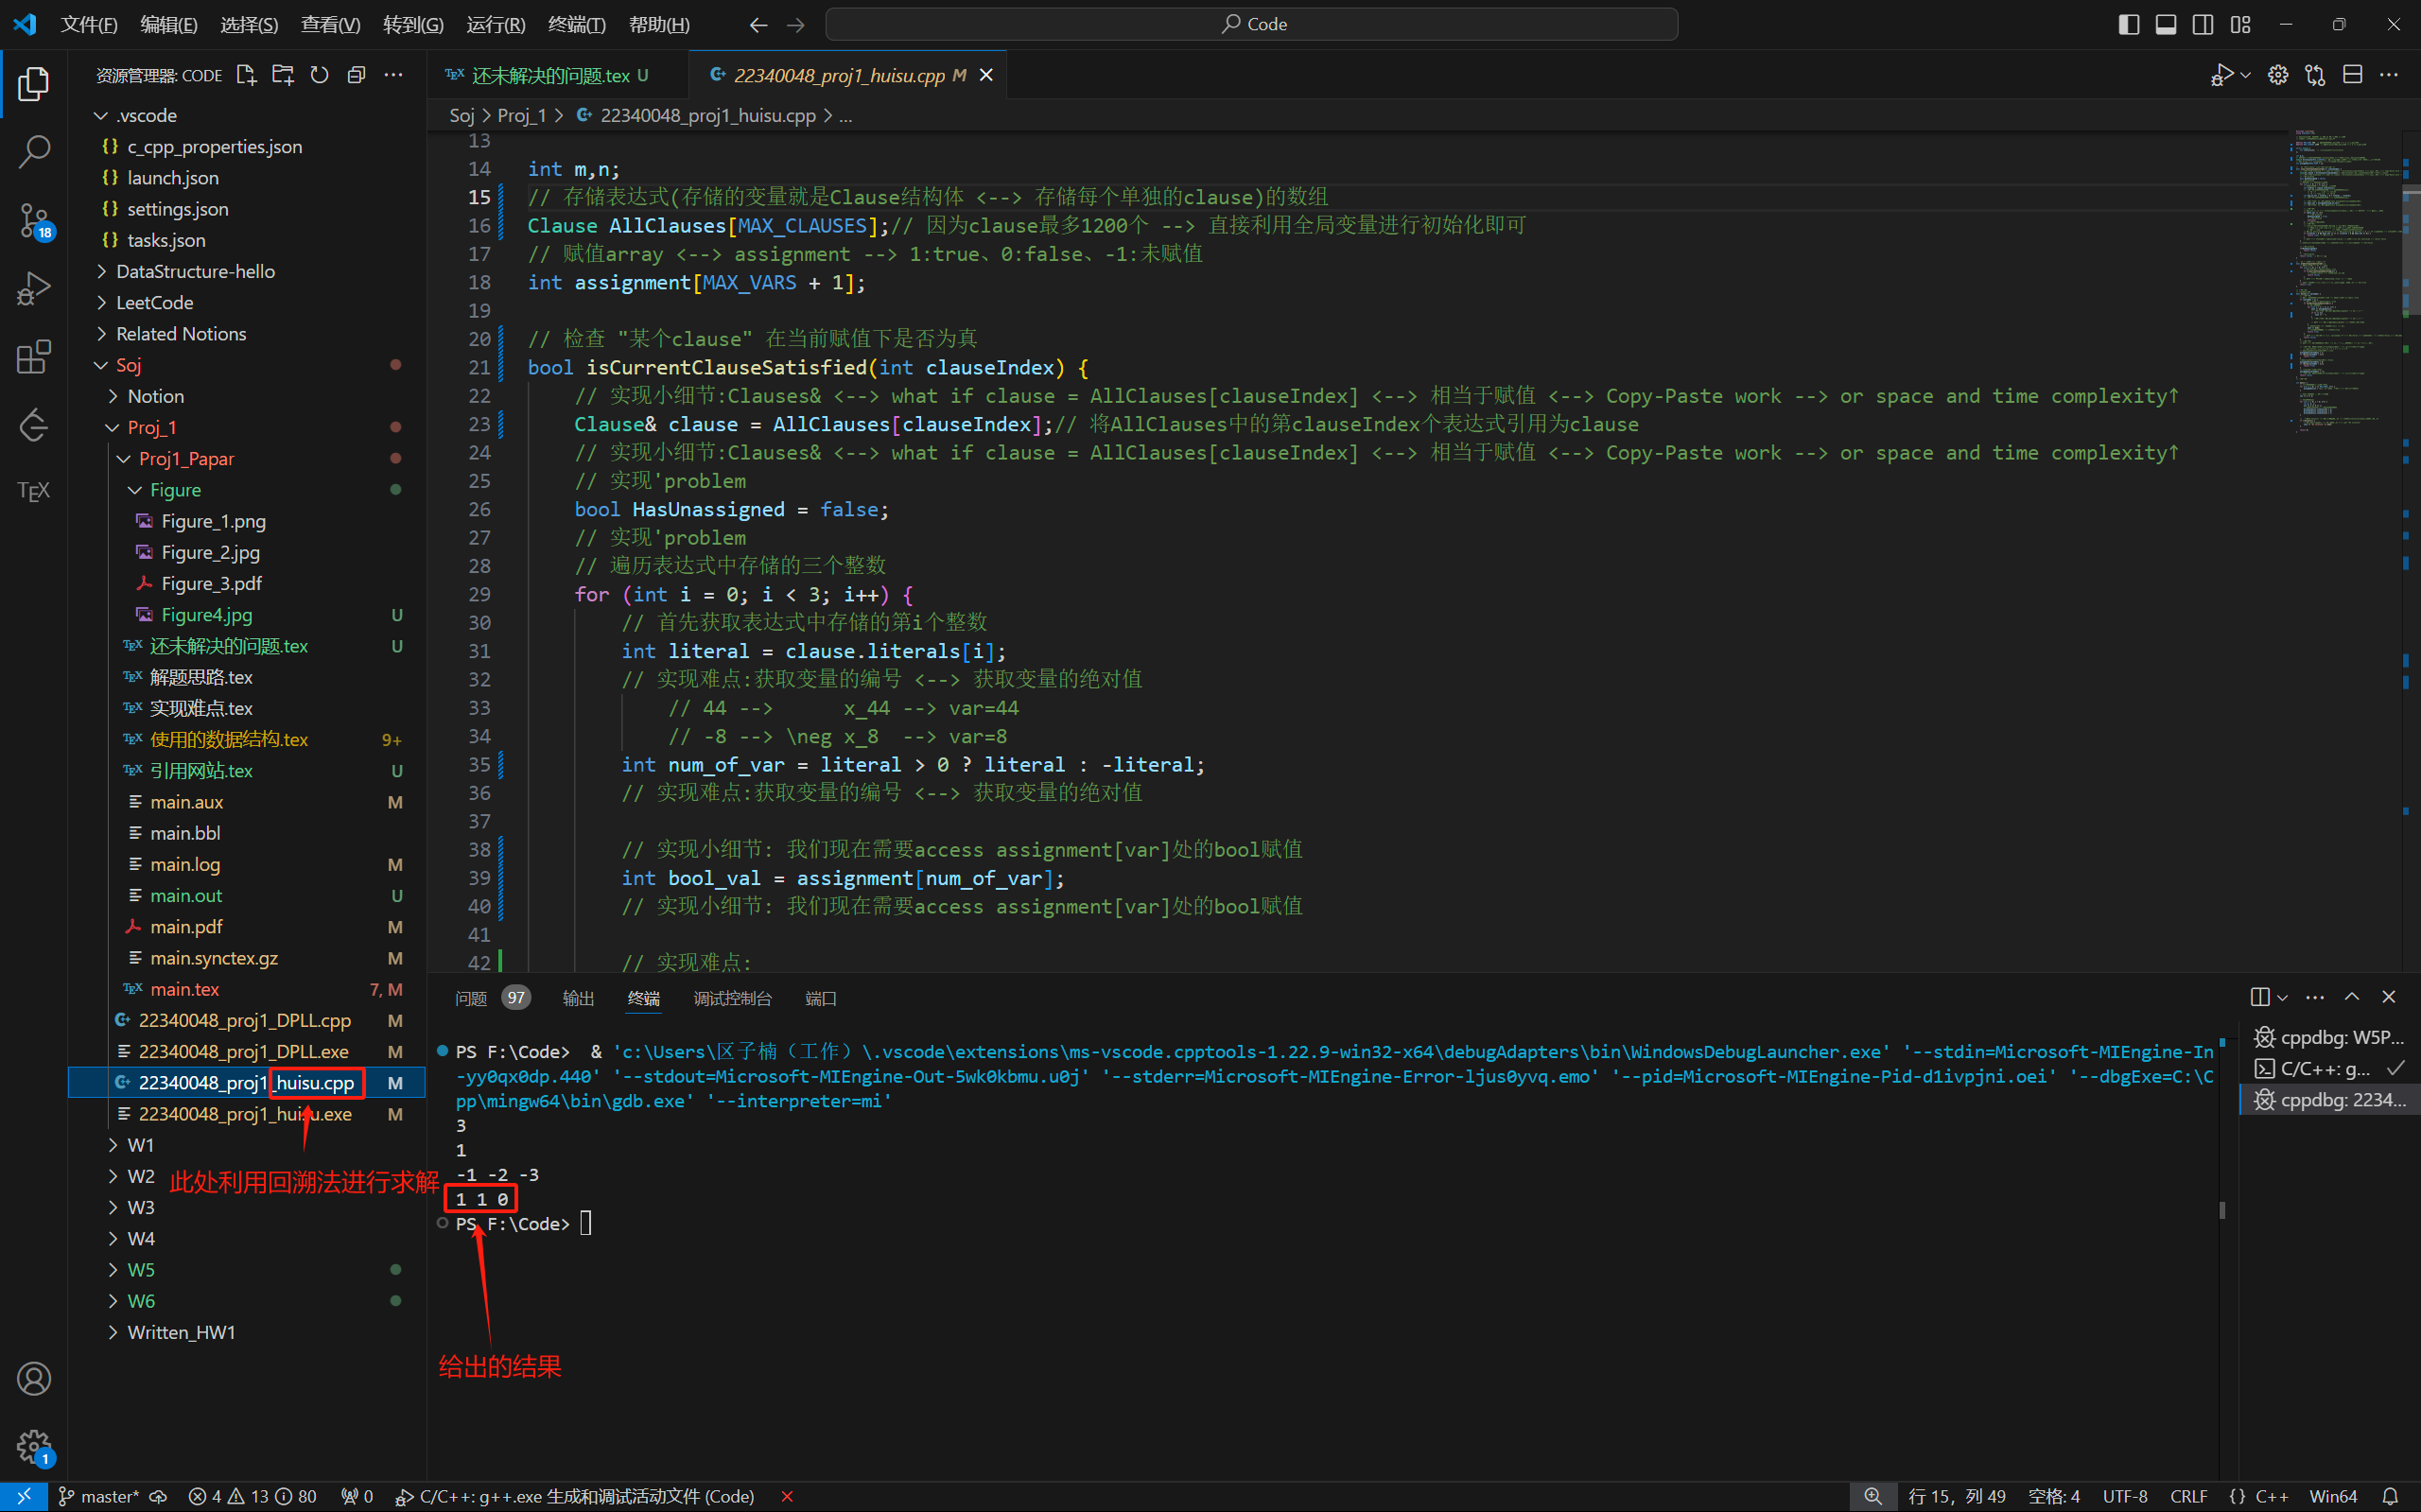
\includegraphics[width=10cm]{Figure/Figure_5.jpg}
        \caption{回溯法求解短测例给出的结果}
    \end{figure}
    \par
    这是利用DPLL算法求解短测例给出的结果
    \begin{figure}[H]
        \centering
        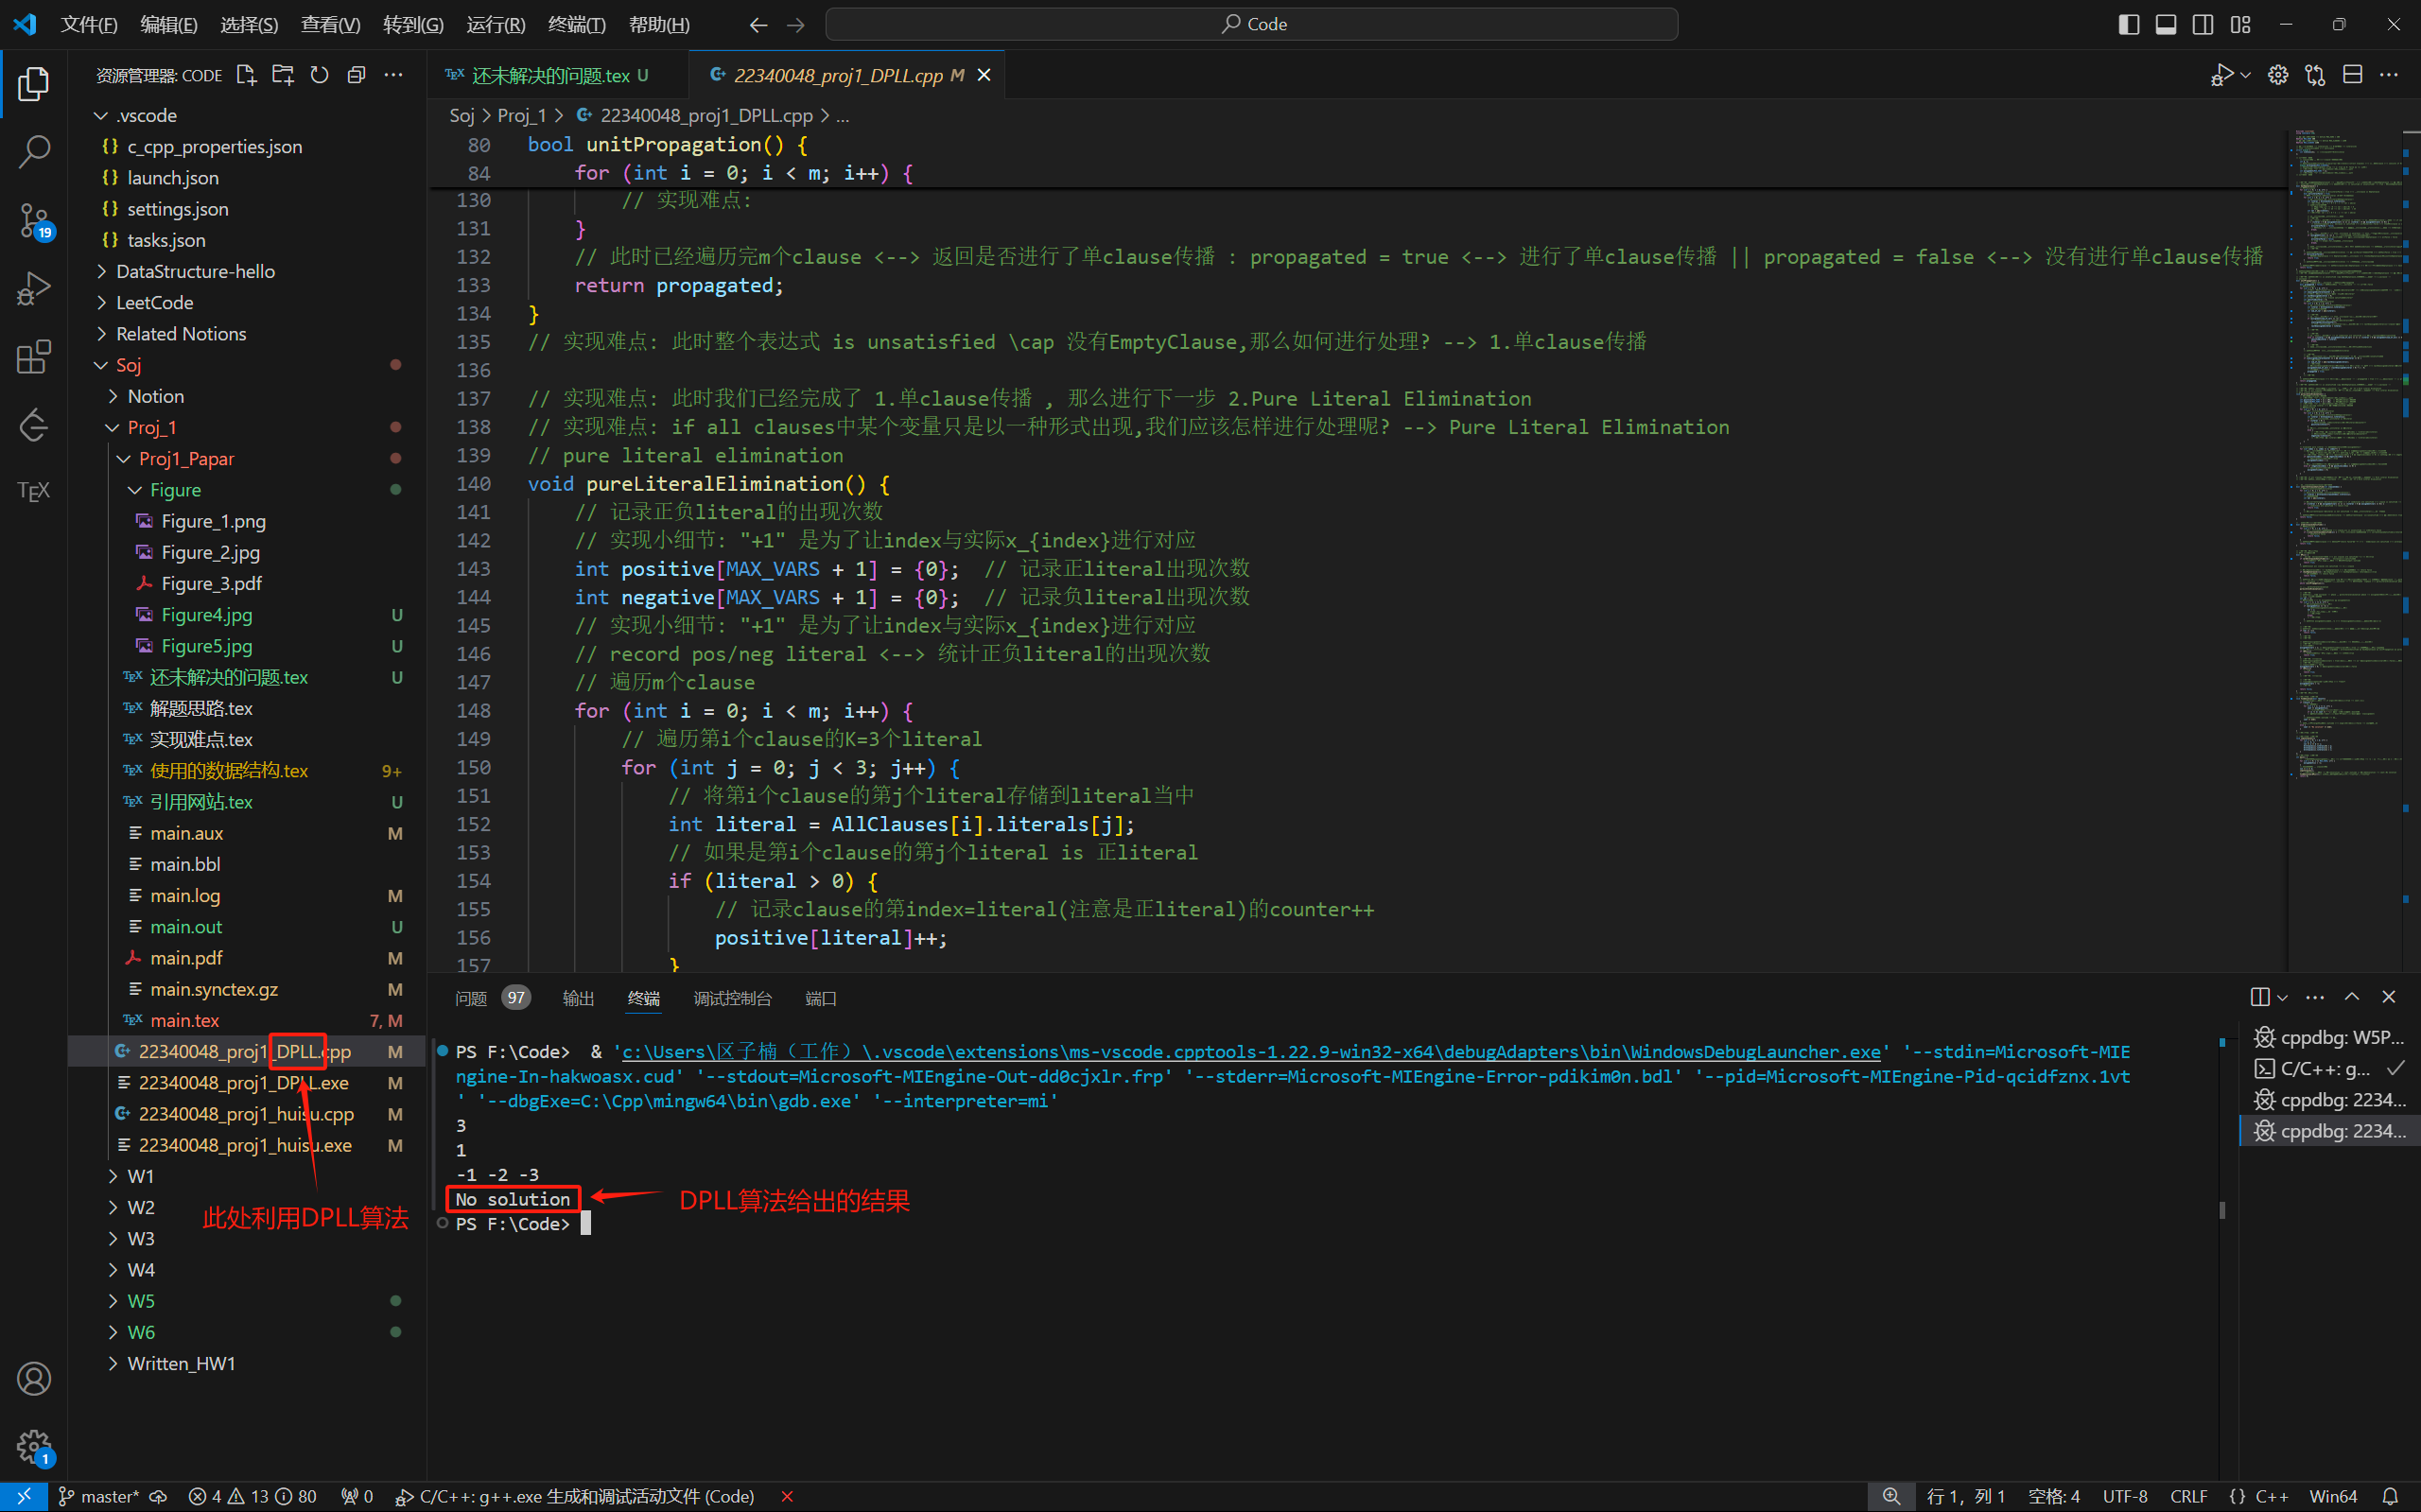
\includegraphics[width=10cm]{Figure/Figure_6.jpg}
        \caption{DPLL算法求解短测例给出的结果}
    \end{figure}
    \par
    很明显现在的这个DPLL算法还是有点小bug的,但是现在还没找出来,留到以后再进行完善。
    \subsection{长测例}
    \par
    考虑如下这么一个例子
    (这里我只放应该得到的结果,实际数据我放在了本地电脑上,如果老师需要我补充数据我也可以提供)
    \begin{figure}[H]
        \centering
        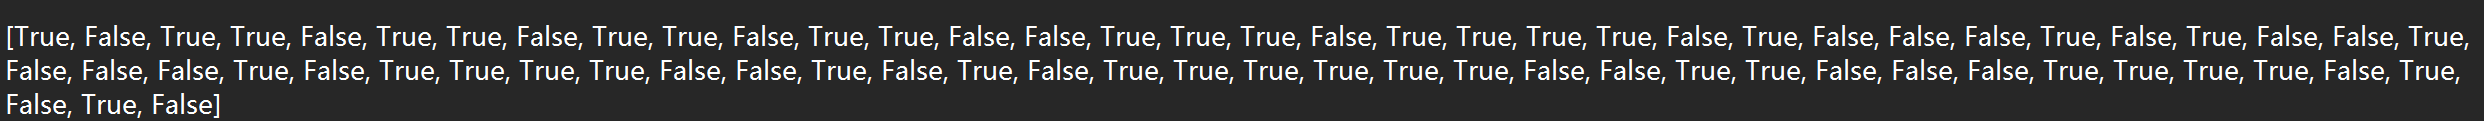
\includegraphics[width=10cm]{Figure/Figure_7.jpg}
        \caption{理论上应该得到的结果}
    \end{figure}
    \par
    这是我利用DPLL算法求解长测例得到的结果
    \begin{figure}[H]
        \centering
        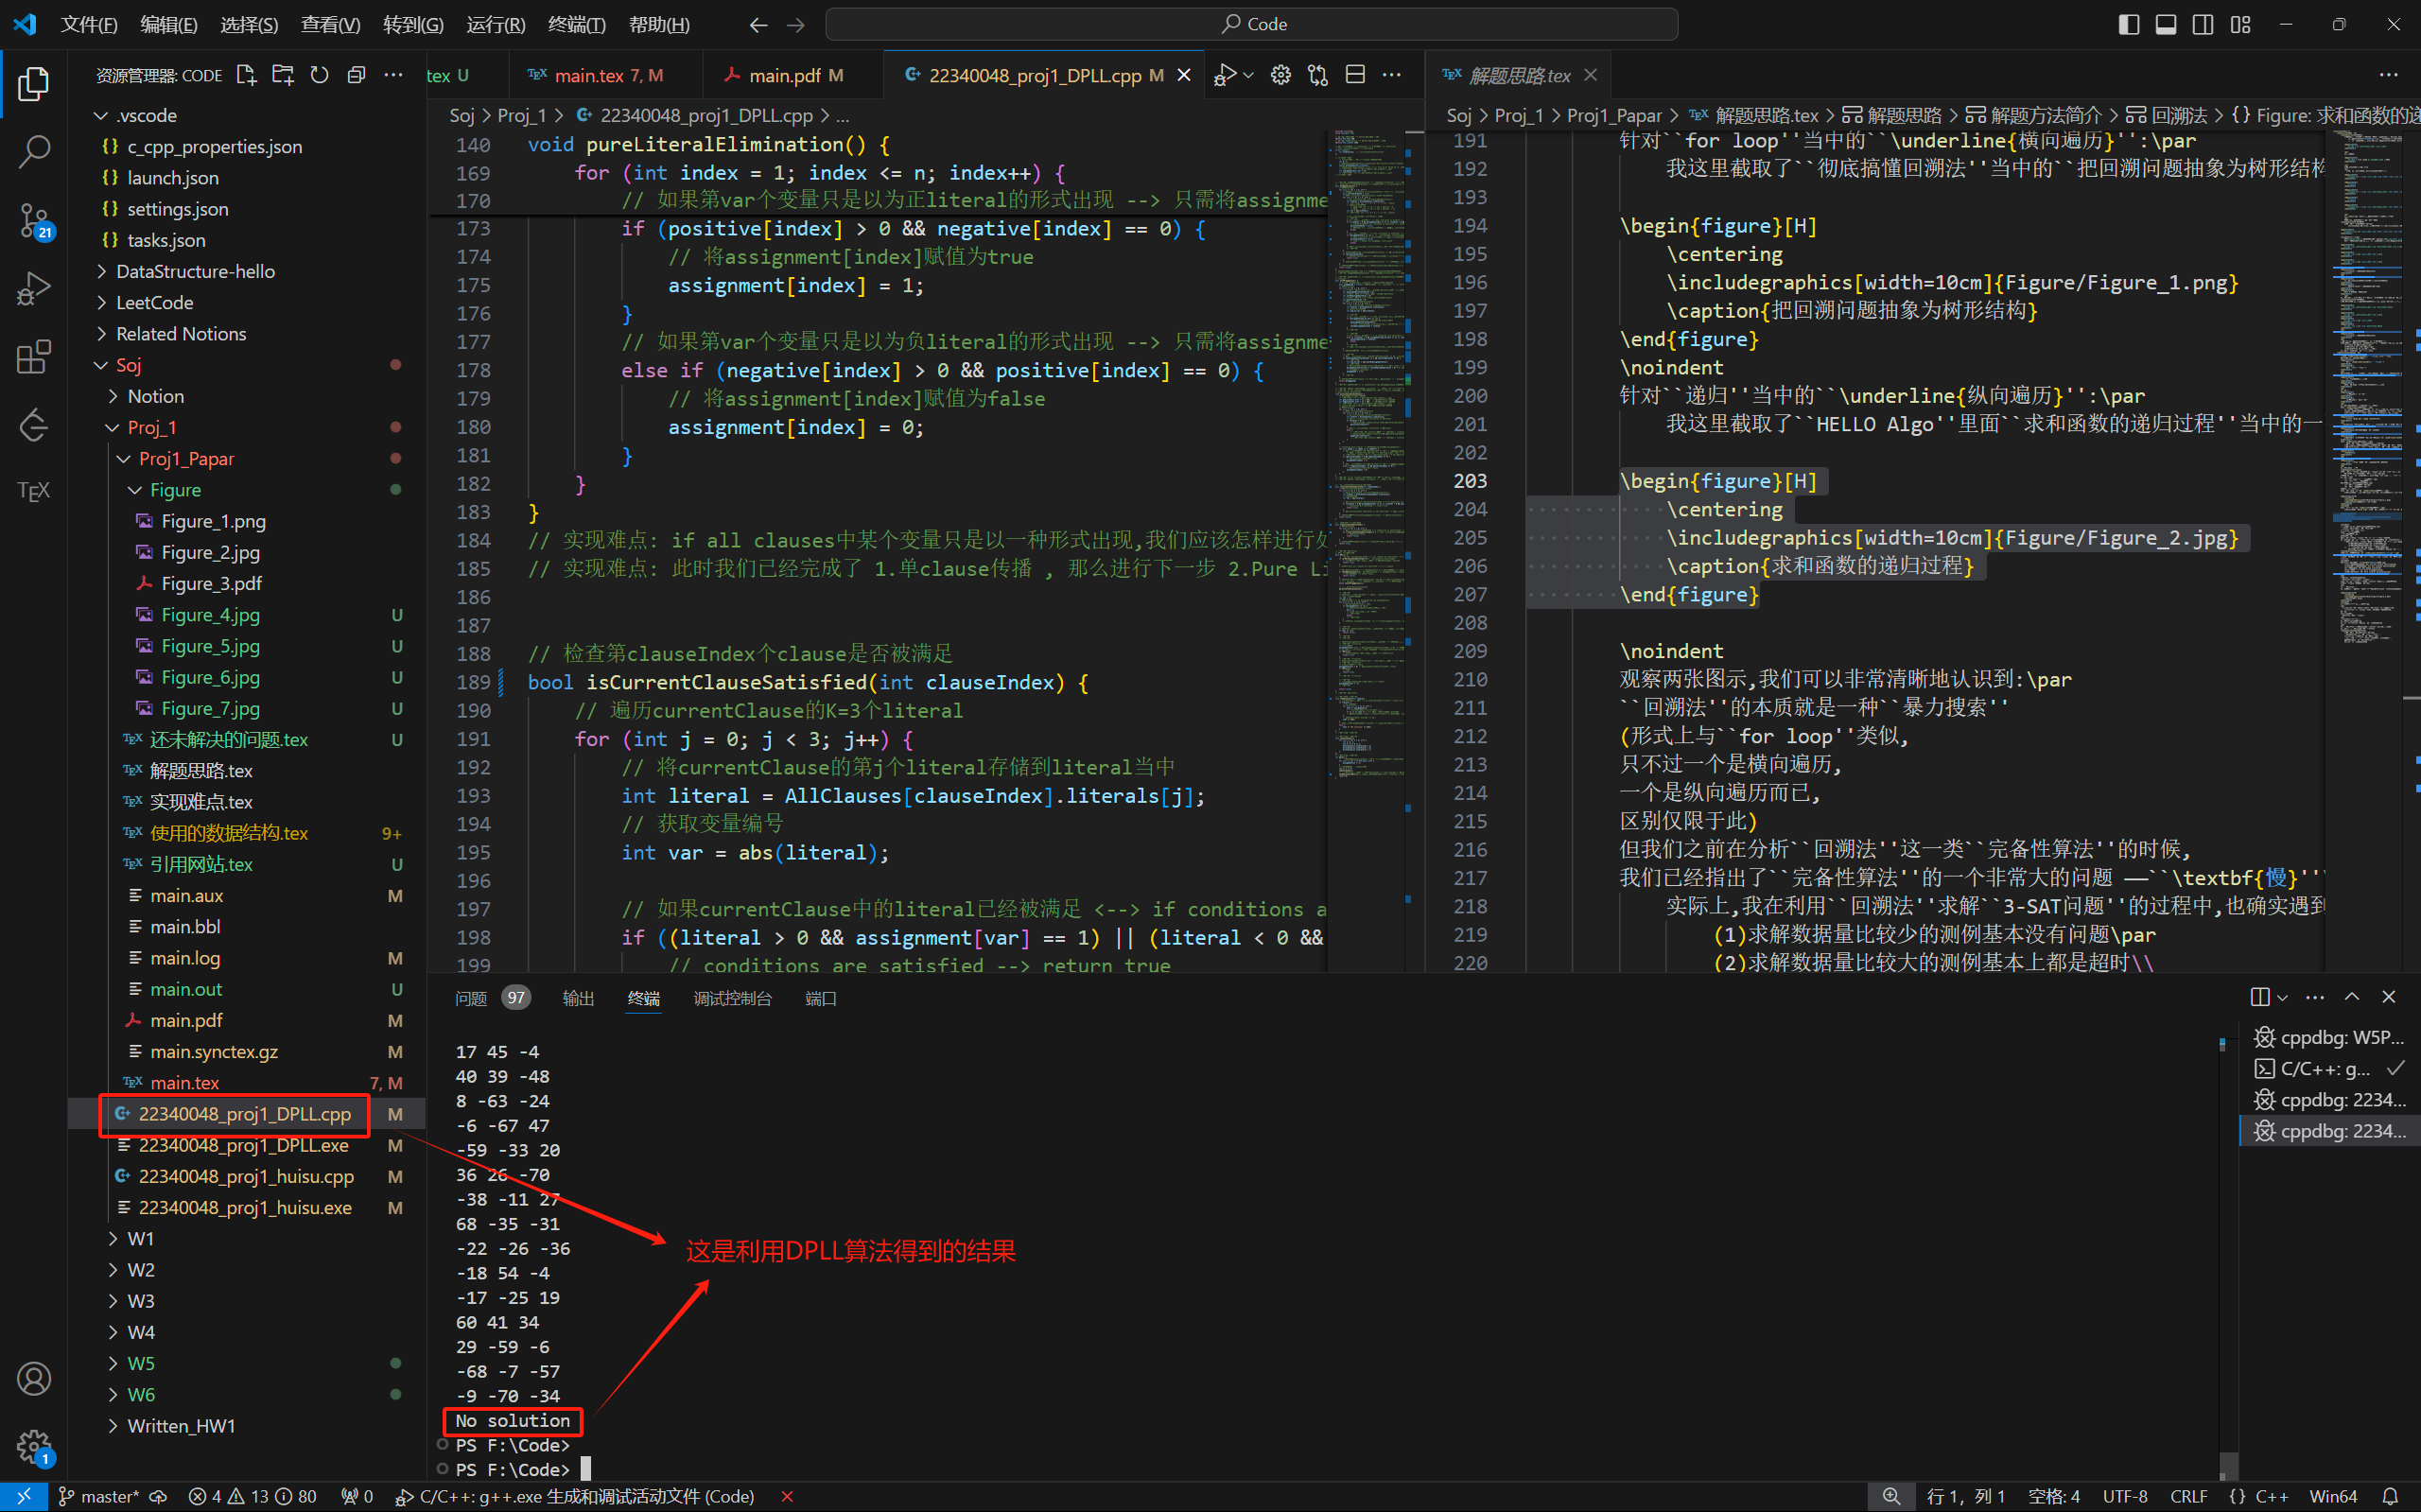
\includegraphics[width=10cm]{Figure/Figure_8.jpg}
        \caption{DPLL算法求解短测例给出的结果}
    \end{figure}
    \par
    同样地,这个长测例也说明了现在的这个DPLL算法还存在一些小漏洞。

